
Operating systems expose an interface that is typically stable and well documented.
%
This engenders a \emph{modeling} approach to the environment problem, which only involves the one-time effort to produce such a model.
%
However, modern operating systems are complex and provide a wide set of abstractions to programs, such as processes and threads, IPC, networking, and files.  Modeling these abstractions is challenging.

In this chapter, we present an approach to modeling the operating system interface that relies on \emph{splitting} the model in a set of most primitive operating system abstractions, on top of which a full operating system model can be implemented with reasonable effort (Section~\ref{sec:cloud9:splitmodel}).
%
We leverage the operating system model to expose hard-to-reproduce scenarios in program execution by providing a \emph{symbolic test} interface for developers (Section~\ref{sec:cloud9:symtests}).
%
Finally, we report on our experience applying these principles when building a POSIX operating system model with support for threads, processes, sockets, pipes, polling, and more (Section~\ref{sec:cloud9:posix}).


\section{Splitting Operating System Environment in Built-in Primitives and Guest Model}
\label{sec:cloud9:splitmodel}
In this section, we first present the design space of an operating system model (Section~\ref{sec:cloud9:modelspace}).  We then present our approach of a split model (Section~\ref{sec:cloud9:approach}) and how we leverage it using symbolic tests.


\subsection{The Design Space of Operating System Models}
\label{sec:cloud9:modelspace}

The goal of a symbolic model is to simulate the behavior of a real execution environment, while maintaining the necessary symbolic state behind the environment interface.
%
The symbolic execution engine can then seamlessly transition back and forth between the program and the environment.

Writing and maintaining a model can be laborious and prone to error~\cite{s2eSystem}.
%
However, for operating system interfaces, which are typically stable and well documented, investing the time to model them becomes worthwile.

Ideally, a symbolic model would be implemented as code that gets executed by the symbolic execution engine (i.e., guest-level code), substituting the implementation of the operating system and the C library.
%
Such a model can be substantially faster.  For instance, in the Linux kernel, transferring a packet between two hosts exercises the entire TCP/IP networking stack and the associated driver code, amounting to over 30 \kloc.  In contrast, our POSIX model achieves the same functionality in about 1.5 \kloc.  Requirements that complicate a real environment/OS implementation, such as performance and extensibility, can be ignored in a symbolic model.

However, not all operating system abstractions can be directly expressed as guest code.
%
In general, the problematic abstractions are those \emph{incompatible} with the execution model of the symbolic execution engine.
%
For example, providing support for multiple execution threads may not be achievable in the guest of a symbolic execution engine designed to run sequentially, unless the guest can manipulate the current stack and program counter.
%
There are other abstractions incompatible with the typical sequential single-process execution model of a symbolic execution engine, such as processes, synchronization, and shared memory.

A possible alternative is to implement the operating system model inside the symbolic execution engine, where we can define any abstraction.
%
However, this approach is undesirable.  A model built into a symbolic execution engine is significantly more expensive to produce, because the model code has to handle explicitly symbolic data and the program state.
%
For example, while a guest model of the \codebit{open} system call could directly use the string buffer of the file name passed as argument, a built-in model needs to explictly invoke read operations for the string bytes, then extract the character values from the symbolic AST expressions.


\subsection{A Split Operating System Model}
\label{sec:cloud9:approach}

Our key idea is to take the best from both worlds and provide an operating system model that is \emph{split} between a set of built-in primitives and guest-level code.
%
The built-in primitives model only the minimal operating system abstractions that would be more expensive or impossible to model at the guest level.
%
In turn, the guest-level code implements a complete operating system interface on top of these primitives.
%
In analogy to the system calls exposed by an operating system to user programs, the symbolic execution engine provides its primitives to the guest through a set of ``symbolic system calls''.

The built-in primitives provide the operating system abstractions that depend on the execution model of the symbolic execution engine.
%
The execution model includes aspects such as the program memory model and the control flow mechanisms.
%
For performance reasons, these aspects are typically encoded in the logic of the symbolic execution engine.

We identified two abstractions that are prevalent in operating systems and that should be built into the symbolic execution engine: \emph{multithreading} and \emph{address spaces}.
%
Multithreading is best provided as a built-in primitive that is integrated with the control flow mechanisms of the symbolic execution engine.
%
Similarly, providing multiple isolated address spaces is best provided by the memory model of the symbolic execution engine.  For example, the functionality needed to support address spaces (e.g., cloning) is shared with the requirements of cloning the execution state after a symbolic branch.

Many other common abstractions do not need to be built into the symbolic execution engine, but can be emulated as guest code on top of threads and address spaces.
%
Such derived abstractions include mechanisms for inter-process communication, such as sockets, pipes and files.
%
Various synchronization mechanisms, such as mutexes, semaphores, condition variables, and barriers can be provided on top of basic multi-threading primitives that put a thread to sleep and wake it up later.

We designed the support for multithreading and address spaces according to two goals: (1) minimizing the complexity of the guest code using them, and (2) capturing all possible behaviors in the real operating system, including corner-case, hard-to-reproduce scenarios.
%
The latter is especially relevant when using the symbolic execution engine to find bugs occurring in the program interaction with the operating system, as we later show in the evaluation (Section~\ref{sec:eval:bug-finding}).


\subsection{Built-in Primitives: Multithreading and Address Spaces}

We next describe the design of multithreading support and address spaces in a symbolic execution engine.

\paragraph{Multithreading}

%% A symbolic execution engine is essentially an interpreter of program statements.
%% %
To provide support for multiple threads, the symbolic execution engine maintains in each execution state a set of per-thread stacks, holding the current program location, the execution call chain, and local variables.
%
During symbolic execution, the execution alternates between the threads, governed by a thread scheduler built into the symbolic execution engine.

To simplify synchronization inside the guest model, we use a cooperative scheduler.  An enabled thread runs uninterrupted (atomically), until either (a) the thread goes to sleep, (b) the thread is explicitly preempted, or (c) the thread is terminated with a symbolic system call.

The scheduler can be configured to schedule the next thread deterministically, or to fork the execution state for each possible next thread.
%
The latter case is useful when looking for concurrency bugs.  At the same time, it can be a significant source of path explosion, so it can be selectively disabled when not needed.

The symbolic execution engine can detect hangs in the system, such as deadlocks, when a thread goes to sleep and no other thread can be scheduled.

\paragraph{Address Spaces}

In symbolic execution, program memory is typically represented as a mapping from memory locations (e.g., variables or addresses) to slots holding symbolic expressions.
%
To provide support for address spaces, we built into the symbolic execution engine support for multiple such mappings per execution state.

Each thread in the execution state is bound to one address space and each address space with its threads forms a process in the execution state.

The symbolic execution engine provides a symbolic system call for \emph{sharing} slots among multiple memory mappings.  This mechanism provides the foundation for implementing shared memory across multiple processes.
%
Shared memory can be used by the guest model to provide multiple forms of inter-process communication, such as sockets, files, and pipes.
%
For example, a socket can be modeled as a pair of memory buffers, one of each direction, shared between the client and the server processes.


\paragraph{Symbolic System Calls}

Table~\ref{table:cloud9:primitives} shows the symbolic system calls that the engine provides to the guest to support multithreading and address spaces.  We detail below the most important system calls.

\begin{table}
\centering
  
\begin{tabular}{|l|l|}
\hline
\textbf{Primitive Name} & \textbf{Description} \\
\hline
\hline
 \codebit{thread\_create(\&func)} & Create new thread that runs \codebit{func} \\
 \codebit{thread\_terminate()} & Terminate current thread \\
\hline
 \codebit{thread\_preempt()} & Preempt the current thread  \\
\hline
 \codebit{create\_wqueue()} & Create a new waiting queue \\
 \codebit{thread\_sleep(wq)} & Put current thread to sleep on waiting queue \\
 \codebit{thread\_notify(wq)} & Wake threads from waiting queue \\
\hline
\hline
 \codebit{process\_fork()} & Fork the current address space and thread \\
 \codebit{make\_shared(\&buf, size)} & Share memory across address spaces \\
\hline
\hline
 \codebit{get\_context()} & Get the current context (process and thread ID) \\
\hline
\end{tabular}

\caption{Symbolic system calls for multithreading (first block), address spaces (second block).  Third block contains introspection primitives.  The multithreading block is further divided into thread lifecycle management, explicit scheduling, and synchronization.}
\label{table:cloud9:primitives}
\end{table}

Threads are created in the currently executing process by calling \codebit{thread\_\allowbreak{}create}.  For instance, the POSIX threads (pthreads) model makes use of this primitive in its own \codebit{pthread\_create()} routine.
%
When \codebit{thread\_sleep} is called, the symbolic execution engine places the current thread on a specified waiting queue, and an enabled thread is selected for execution.
%
Another thread may call \codebit{thread\_\allowbreak{}notify} on the waiting queue and wake up one or all of the queued threads.

Cloning the current address space is available to the guest through the \codebit{process\_fork} primitive, which is used, for instance, to model the POSIX \codebit{fork()} call.
%
A memory location can be marked as shared by calling \codebit{make\_\allowbreak{}shared}; it is then automatically mapped in the address spaces of the other processes in the execution state.  Whenever a shared object is modified in one address space, the new version is automatically propagated to the others.


%%% Local Variables: 
%%% mode: latex
%%% eval: (visual-line-mode)
%%% fill-column: 1000000
%%% TeX-master: "main"
%%% End:


\section{Symbolic Tests}
\label{sec:cloud9:symtests}
Software products and systems typically have large ``hand-made'' test suites; writing and maintaining these suites requires substantial human effort.
%
\cnine aims to reduce this burden while improving the quality of testing, by offering an easy way to write ``symbolic test suites.''
%
First, a symbolic test case encompasses many similar concrete test cases into a single symbolic one---each symbolic test a developer writes is equivalent to many concrete ones.
%
Second, a symbolic test case explores conditions that are hard to produce reliably in a concrete test case, such as the occurrence of faults, concurrency side effects, or network packet reordering, dropping and delay.
%
Furthermore, symbolic test suites can easily cover unknown corner cases, as well as new, untested functionality.  In this section, we present the API for symbolic tests and illustrate it with a use case.

\subsection{Testing Platform Interface}

The \cnine symbolic testing API (Tables~\ref{table:globalapi} and~\ref{table:ioctlapi}) allows tests to programmatically control events in the environment of the program under test.
%
A test suite needs to simply include a \codebit{cloud9.h} header file and make the requisite calls.

\begin{table}
\addtolength{\tabcolsep}{-2.5pt}
{
\small
\centering
\begin{tabular}{|l|p{50mm}|}
\hline
\textbf{~~~~~Function Name} & \textbf{~~~~~~~~~~~~~~~~~~Description} \\
\hline
\cninesuffix\_make\_symbolic & Mark memory regions as symbolic \\
\hline
\cninesuffix\_fi\_enable & \multirow{2}{4cm}{Enable/disable the injection of faults} \\
\cninesuffix\_fi\_disable & \\
\hline
\cninesuffix\_set\_max\_heap & Set heap size for symbolic \codebit{malloc} \\
\hline
\cninesuffix\_set\_scheduler & Set scheduler policy (e.g., round-robin)\\
\hline
\end{tabular}
\vspace{-4pt}
\caption{\cnine API for setting global behavior parameters.}
\label{table:globalapi}
}
\end{table}

\begin{table}
\addtolength{\tabcolsep}{-2.5pt}
{
\small
\centering
\begin{tabular}{|l|p{4.8cm}|}
\hline
\textbf{~~Extended Ioctl Code} & \textbf{~~~~~~~~~~~~~~~~Description} \\
\hline
SIO\_SYMBOLIC & Turns this file or socket into a source of symbolic input \\
\hline
SIO\_PKT\_FRAGMENT & Enables packet fragmentation on this socket (must be a stream socket) \\
\hline
SIO\_FAULT\_INJ & Enables fault injection for operations on this descriptor \\
\hline
\end{tabular}
\vspace{-4pt}
\caption{\cnine extended \codebit{ioctl} codes to control environmental events on a per-file-descriptor basis.}
\label{table:ioctlapi}
}
\end{table}

\paragraph{Symbolic Data and Streams}

The generality of a test case can be expanded by introducing bytes of symbolic data.
%
This is done by calling \codebit{\cninesuffix\_make\_symbolic} to mark data symbolic, a wrapper around the SEE's primitive for injecting fresh symbolic variables in the program state.
%
%% a wrapper around \codebit{klee\_\allowbreak{}make\_\allowbreak{}symbolic}, with an argument that points to a memory region. \codebit{klee\_make\_symbolic} is a primitive provided by \klee to mark data symbolic.
%
In addition to wrapping this call, we added several new primitives to the testing API (Table~\ref{table:globalapi}). In \cnine, symbolic data can be written/read to/from files, can be sent/received over the network, and can be passed via pipes. Furthermore, the \codebit{SIO\_SYMBOLIC} \codebit{ioctl} code (Table~\ref{table:ioctlapi}) turns on/off the reception of symbolic bytes from individual files or sockets.

\paragraph{Network Conditions}

Delay, reordering, or dropping of packets causes a network data stream to be fragmented.
%
Fragmentation can be turned on or off at the socket level using one of the \cnine \codebit{ioctl} extensions.  Section~\ref{sec:eval:lighttpd} presents a case where symbolic fragmentation enabled \cnine to prove that a bug fix for the lighttpd web server was incomplete. 

\paragraph{Fault Injection}

Calls in a POSIX system can return an error code when they fail.
%
Most programs can tolerate such failed calls, but even high-quality production software misses some~\cite{lfi}. Such error return codes are simulated by \cnine whenever fault injection is turned on. 

\paragraph{Symbolic Scheduler}

\cnine provides multiple scheduling policies that can be controlled for purposes of testing on a per-code-region basis.
%
Currently, \cnine supports a round-robin scheduler and two schedulers specialized for bug finding: a variant of the iterative context bounding scheduling algorithm~\cite{chess} and an exhaustive exploration of all possible scheduling decisions.  


\subsection{Usage Example: Testing Custom Header Handling in Web Server}

Consider a scenario in which we want to test the support for a new \codebit{X-NewExtension} HTTP header, just added to a web server.
%
We show how to write tests for this new feature.

A symbolic test suite typically starts off as an augmentation of an existing test suite;
%
in our scenario, we reuse the existing boilerplate setup code and write a symbolic test case that marks the extension header symbolic. Whenever the code that processes the header data is executed, \cnine forks at all the branches that depend on the header content. Similarly, the request payload can be marked symbolic to test the payload-processing part of the system:

\begin{verbatim}
   char hData[10];
   cloud9_make_symbolic(hData);
   strcat(req, "X-NewExtension: ");
   strcat(req, hData);
\end{verbatim}

The web server may receive HTTP requests fragmented in a number of chunks, returned by individual invocations of the \codebit{read()} system call---the web server should run correctly regardless of the fragmentation pattern.
%
To test different fragmentation patterns with \cnine, one simply enables symbolic packet fragmentation on the client socket:
\begin{verbatim}
   ioctl(ssock, SIO_PKT_FRAGMENT, RD);
\end{verbatim}

To test how the web server handles failures in the environment, we can ask \cnine to selectively inject faults when the server reads or sends data on a socket by placing in the symbolic test suite calls of the form:
\begin{verbatim}
   ioctl(ssock, SIO_FAULT_INJ, RD | WR);
\end{verbatim}
\cnine can also enable/disable fault injection globally for all file descriptors within a certain region of the code using calls to \codebit{\cninesuffix\_fi\_\allowbreak{}enable} and \codebit{\cninesuffix\_fi\_\allowbreak{}disable}. For simulating low-memory conditions, \cnine provides a \codebit{\cninesuffix\_set\_\allowbreak{}max\_heap} primitive, which can be used to test the web server with different maximum heap sizes.

%%% Local Variables: 
%%% mode: latex
%%% eval: (visual-line-mode)
%%% fill-column: 1000000
%%% TeX-master: "main"
%%% End:


\section{Case Study: A Symbolic POSIX Interface Model}
\label{sec:cloud9:posix}
We used the SEE system call interface to build a model for the POSIX interface.
%
In this section, we describe the key design decisions involved in building the model, and we illustrate the use of the symbolic system call interface.
%
This also serves as an example for building additional models on top of the \cnine symbolic system call interface.

The POSIX model uses shared memory structures to keep track of all system objects (processes, threads, sockets, etc.).
%
The two most important data structures are stream buffers and block buffers, analogous to character and block device types in UNIX.  Stream buffers model half-duplex communication channels: they are generic producer-consumer queues of bytes, with support for event notification to multiple listeners.  Event notifications are used, for instance, by the polling component in the POSIX model.  Block buffers are random-access, fixed-size buffers, whose operations do not block; they are used to implement symbolic files.

The symbolic execution engine maintains only basic information on running processes and threads: identifiers, running status, and parent--child information.
%
However, the POSIX standard mandates additional information, such as open file descriptors and permission flags. This information is stored by the model in auxiliary data structures associated with the currently running threads and processes. The implementations of \codebit{fork()} and \codebit{pthread\_create()} are in charge of initializing these auxiliary data structures and making the appropriate symbolic system calls.

Modeling synchronization routines is simplified by the cooperative scheduling policy:
%
no locks are necessary, and all synchronization can be done using the sleep/notify symbolic system calls, together with reference counters.  Figure~\ref{fig:mutexcode} illustrates the simplicity this engenders in the implementation of pthread mutex lock and unlock.

\begin{figure}
  \centering
  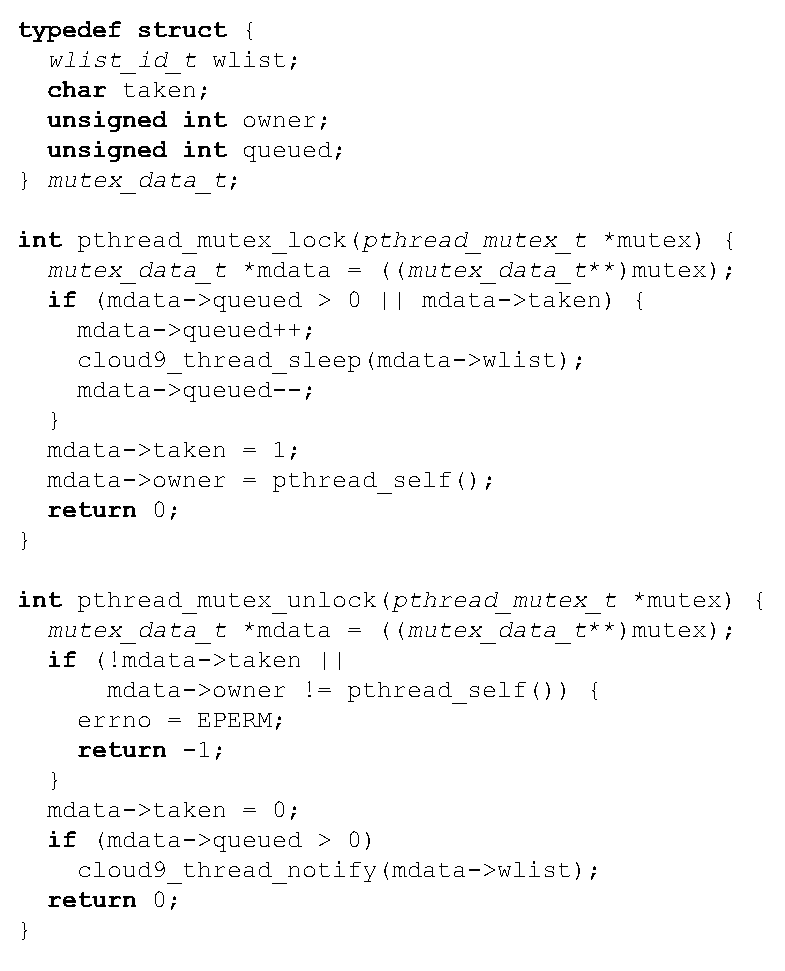
\epsfig{file=cloud9/figures/mutex-model.eps, width=3.2in}
  \caption{Example implementation of pthread mutex operations in \cnine's POSIX environment model.}
  \label{fig:mutexcode}
\end{figure}

\cnine uses most of \klee's file model semantics.
%
In particular, one can either open a symbolic file (its contents comes from a symbolic block buffer), or a concrete file, in which case a concrete file descriptor is associated with the symbolic one, and all operations on the file are forwarded as external calls on the concrete descriptor. 

\begin{figure}
  \centering
  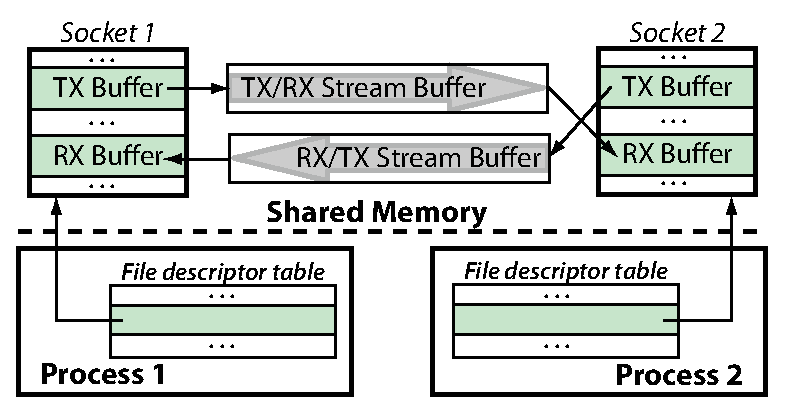
\epsfig{file=cloud9/figures/network-model.eps, width=4.0in}
  \caption{A TCP network connection is modeled in \cnine using TX and RX buffers implemented as stream buffers.}
  \label{fig:networkmodel}
\end{figure}

In addition to file objects, the \cnine POSIX model adds support for networking and pipes.
%
Currently, the TCP and UDP protocols are supported over IP and UNIX network types. Since no actual hardware is involved in the packet transmission, we can collapse the entire networking stack into a simple scheme based on two stream buffers (Figure~\ref{fig:networkmodel}). The network is modeled as a single-IP network with multiple available ports---this configuration is sufficient to connect multiple processes to each other, in order to simulate and test distributed systems. The model also supports pipes through the use of a single stream buffer, similar to sockets.

The \cnine POSIX model supports polling through the \codebit{select()} interface.
%
All the software we tested can be configured to use \codebit{select()}, so it was not necessary to implement other polling mechanisms.  The \codebit{select()} model relies on the event notification support offered by the stream buffers that are used in the implementation of blocking I/O objects (currently sockets and pipes).

The constraint solver used in \cnine operates on bit vectors; as a result, symbolic formulas refer to contiguous areas of memory.
%
In order to reduce the constraint solving overhead, we aim to reduce the amount of intermixing of concrete and symbolic data in the same memory region.  Thus, \cnine's POSIX model segregates concrete from symbolic data by using static arrays for concrete data and linked lists (or other specialized structures) for symbolic data.  We allocate into separate buffers potentially-symbolic data passed by the tested program through the POSIX interface.

In order to enable testing the systems presented in the evaluation section (Section~\ref{sec:eval:targets}), we had to add support for various other components: IPC routines, \codebit{mmap()} calls, time-related functions, etc.
%
Even though laborious, this was mostly an engineering exercise, so we do not discuss it further.

Finally, in some cases, it is practical to have the host OS handle parts of the environment via \emph{external calls}.
%
These are implemented by concretizing the symbolic parameters of a system call before invoking it from symbolically executing code. Unlike \cite{dart,klee,exe}, \cnine allows external calls \emph{only} for stateless or read-only system calls, such as reading a system configuration file from the \codebit{/etc} directory.  This restriction ensures that external concrete calls do not clobber other symbolically executing paths.

%%% Local Variables: 
%%% mode: latex
%%% eval: (visual-line-mode)
%%% fill-column: 1000000
%%% TeX-master: "main"
%%% End:


\section{Summary}

Operating systems expose a complex stateful interface to user programs.
%
In this chapter, we showed a way to provide an operating system environment for symbolic execution by employing a split operating system model.  A core set of primitives built into the symbolic execution engine serves as a base, on top of which a full operating system interface is emulated inside the guest.
%
As few as two primitives are sufficient to support complex operating system interfaces: threads  with synchronization and address spaces with shared memory.
%
We showed how to use the core primitives to provide an accurate model of the POSIX interface.
%
Our POSIX model includes extensions that developers can use in symbolic tests to control non-deterministic operating system events, such as thread scheduling and network flow control, in order to increase the coverage in the target programs.

%%% Local Variables: 
%%% mode: latex
%%% eval: (visual-line-mode)
%%% fill-column: 1000000
%%% TeX-master: "main"
%%% End:
